\documentclass[unicode, 12pt, aspectratio=169]{beamer}
\usetheme{boxes}
\usepackage{luatexja}
\usepackage{ifxetex,ifluatex}
\usepackage{unicode-math}
\usepackage{graphicx, amsmath, cite, ascmac, amsfonts}
\renewcommand{\kanjifamilydefault}{\gtdefault}
\makeatletter
\newcommand{\tref}[1]{Table.~\ref{#1}}
\newcommand{\eref}[1]{Eq.~(\ref{#1})}
\newcommand{\fref}[1]{Fig.~\ref{#1}}
\renewcommand{\theequation}{
  \thesection.\arabic{equation}}
\@addtoreset{equation}{chapter}
\def\cite#1{\textsubscript{#1}}
%\def\section{\newpage\@startsection {section}{2}{\z@}{3truemm}{3truemm}{\Large\bf}}
\makeatother
%\AtBeginSection[]{
%  \frame{\tableofcontents[currentsection, hideallsubsections]}
%}

\author{前田大輝}
\title{周期ポテンシャルにおける波束の時間発展}
\begin{document}
\frame{\maketitle}
\begin{frame}
\tableofcontents
\end{frame}
\section{概要}
\frame{\insertsection}
\begin{frame}
    \begin{itemize}
      \item 周期ポテンシャル:周期構造をモデル化
      \item Kronig-Pennyモデル:エネルギーバンド構造
      \item 波束:局在化した波
      \item 本研究:(半)周期ポテンシャルにおける波束がどのように緩和していくのか
      \item 方法:コンピュータで数値計算
    \end{itemize}
\end{frame}
\section{研究目的}
\begin{frame}
   \begin{block}{物質中の電子:エネルギーバンド構造}
        定常状態での解析はなされている\\
        \alert{but}\\
        時間依存の詳細についてはまだ未解明\\
        \structure{バンドができる時間を知りたい}
   \end{block}
\end{frame}
\subsection{波束}
\frame{\insertsubsection}
\begin{frame}{波束の時間発展}
  \begin{block}{波束とは}
    \begin{itemize}
      \item 局在化した波動
      \item 古典的な質点に対応
      \item ex)電子パルス
    \end{itemize}
  \end{block}
  \begin{block}{古典近似成立条件}
    \begin{align}
      \frac{\delta x}{d} \ll 1\label{acc}
    \end{align}
    古典近似は時間とともに成立しなくなる
  \end{block}
\end{frame}

\begin{frame}{古典近似}
  \begin{block}{自由量子波束}
    → 時間依存した現象\\
    Schrödinger方程式における静止自由波束は時間とともに緩和\\
    →\eref{acc}が成立しなくなる
  \end{block}
  \begin{block}{目安}
  \begin{align}
     \sigma(t) = \sigma_0 + \alpha t\label{SD}
   \end{align}
  \end{block}
\end{frame}

\begin{frame}{古典近似}
  \begin{block}{\eref{acc}の陽に時間依存した形}
    \begin{align}
      \frac{\sigma_0 + \alpha t}{d} \ll 1
    \end{align}
    成立時間
    \begin{align}
      \delta t_{lim} \sim \frac{d}{\alpha} \label{acc2}
    \end{align}
  \end{block}
    \alert{but}\\\eref{acc2}は前提として力が加わっていない状態\\
    \structure{物質中のポテンシャルについても目安を知りたい}
\end{frame}

\begin{frame}{波束についてのまとめ}
      \begin{itemize}
        \item 波束は古典近似で質点に対応する
        \item 波束は時間発展とともに緩和する
        \item 物質中での緩和速度についてはよくわかっていない
      \end{itemize}
\end{frame}

\subsection{Kronig-Pennyモデル}
\frame{\insertsubsection}
\begin{frame}{Blochの定理}
  \begin{block}{結晶}
    エネルギー固有状態に飛躍がある\\
    →エネルギーバンド構造\\
    →結晶の並進対称性
  \end{block}
   \begin{block}{Blochの定理}
    結晶原子が周期的$\rightarrow$ポテンシャルが周期的\\
    一般的な形式\eref{BlochTheorem}
      \begin{align}
        \phi(x) = u(x) \mathrm{e}^{-k x} \label{BlochTheorem}
      \end{align}
   \end{block}
\end{frame}

\begin{frame}{Kronig-Pennyモデル}
  \begin{block}{Kronig-Pennyポテンシャル}
    \eref{defKP}のように表されるポテンシャルではエネルギーバンド構造が形成
    \begin{align}
        V_{KP}(x) =
        \begin{cases}
          V_0  & (0 \leq x \leq a)\\
          0    & (a \leq x \leq d)\\
          V_{KP}(x - d) & (otherwise)
        \end{cases}\label{defKP}
      \end{align}
    \end{block}
   箱型ポテンシャルが周期的に並んだ構造\\
   $\rightarrow$周期ポテンシャルの中でも最も単純
    \begin{block}{簡単な構造}
    \alert{but}\\
    エネルギーバンド構造を説明できる
    \end{block}
\end{frame}

\begin{frame}{非定常状態のKronig-Pennyモデル}
  \begin{block}{Kronig-Pennyモデルでは・・・・・・}
    定常状態は古くから知られている\\
      \alert{but}非定常状態はよくわからない
      \alert{because}非定常状態ではBlochの定理が成立しない
  \end{block}

  \begin{block}{Hunagel、Zhangの量子拡散についての研究}
      波束が”強く”緩和\\
      →Heyperdiffusion\\
      \alert{but}\\
      \structure{真空中から物質中に入射する波束については未知}
  \end{block}
\end{frame}

 \begin{frame}{課題}
    結晶に入ると瞬時にエネルギーバンド状態になる近似\\
    \alert{but}\\
    波束:非定常\\
    エネルギーバンド:定常\\
    \structure{一瞬では移り変われない}\\
    \alert{morever}\\
    \structure{エネルギーバンドを作る過程が観測にかかる可能性}\\
    \begin{alertblock}{エネルギーバンド構造が作られる時間を知りたい}
    最も簡単な周期ポテンシャル\rightarrow Kronig-Pennyモデルを使う
    \end{alertblock}
\end{frame}

\begin{frame}
      \begin{itemize}
        \item 物質中の電子は定常状態でエネルギーバンド構造を作る
        \item Kronig-Pennyモデルはエネルギーバンド構造を説明できる
        \item 真空からKronig-Pennyポテンシャルに入射する波束の緩和についてはよくわかっていない
      \end{itemize}
\end{frame}

\section{数値計算}
\subsection{Euler法}
\frame{\insertsubsection}

\begin{frame}{このセクションの目的}
    学部生に数値的に解くことの雰囲気を知ってもらうこと!!
    \begin{alertblock}{数値計算の力強さの源}
     形式的な話$\rightarrow$どんな方程式にも対応できる\\
      \alert{”どんな難しい方程式も解くことができる”}\\
      \structure{大雑把に何をやっているのかを知ってほしい。}
    \end{alertblock}
\end{frame}

\begin{frame}
  \begin{block}{一階の常微分方程式の一般形}
    \begin{align}
      \frac{dy}{dt} = f(y,t)\label{diffEQ1}\\
      y(t_0) = y_0\label{diffEQ2}
    \end{align}
    ここで$y_0$は初期条件として与えられる既知の値
  \end{block}
\end{frame}

\begin{frame}
  \begin{block}{何が大変?}
    \eref{diffEQ1}の右辺を積分$\rightarrow$積分定数として\eref{diffEQ2}\\
    \structure{$\rightarrow$方程式の解が得られる}
    \alert{but}\\
    計算機で数値的に解く際にこの方法は使うことができない\\
    $\rightarrow$計算機は有限回の加減乗除しかできない
  \end{block}
\end{frame}

\begin{frame}
    解析的手段が使えない$\rightarrow$解析解を得る手段がない\\
    解析解を得ることは諦める\\
    任意の精度で真の値に近い値を得ることができればOK\\
    無限回の計算を有限回で打ち切る\\
    \alert{つまり近似!!!}
\end{frame}

\begin{frame}
    近似方法$\rightarrow$たくさんある\\
    この節の目的達成に最も適した方法$\rightarrow$Euler法\\
    あまり実用的ではない\\
    \alert{but}\\
    数値計算の難しさや、力強さを掴んでもらうためには十分
    \begin{alertblock}{理由}
    最も基礎的な計算方法だから\\
      Euler法の発展$\rightarrow$Runge-Kutta法(最もメジャー)
    \end{alertblock}
\end{frame}

\begin{frame}
  $y(t)$を\alert{$t=t_0$}の周りでTaylor展開(プリントは誤字)
  \begin{align}
      y(t) = y(t_0) + \left.\frac{dy}{dt}\right|_{t=t_0}\!(t-t_0) 
      + \frac{1}{2}\left.\frac{d^2y}{dt^2}\right|_{t=t_0}\!(t-t_0)^2 + \dots\label{Ytaylor1}
    \end{align}
\end{frame}

\begin{frame}
  \begin{block}{生き残る項}
    一次の項:\eref{diffEQ1}\\
    ゼロ次の項:\eref{diffEQ2}\\
    二次以降の項は$t=t_0$の近傍で無視できる\\
  \end{block}

  \begin{block}{結果}
    \begin{align}
      y(t_0 + h) \simeq y_0 + f(y_0,0)h = y_1 \label{EulerMethod1} 
    \end{align}
    $h$はステップ幅\\
    既知の値$y_0$から、未知の値$y(t_0 + h)=y_1$を得ることができた
  \end{block}
\end{frame}

\begin{frame}
  \begin{block}{同様に}
    $t=t_0 + h = t_1$の周りでTaylor展開\\
    一次の項:\eref{diffEQ1}\\
    ゼロ次の項:\eref{diffEQ2}\\
    二次以降の項は$t=t_0$の近傍で無視できる\\
    \begin{align}
      y(t_1 + h) \simeq y_1 + f(y_1,t_1)h = y_2\label{EulerMethod2} 
    \end{align}
  \end{block}
    これらの操作を次々に繰り返すことで、$t=t_n$における$y(t)$の値を求めることができる。
\end{frame}

\begin{frame}
    微分方程式\eref{diffEQ1}、\eref{diffEQ2}の解
    \begin{block}{Euler法}
      \begin{align}
        y_{n+1} = y_n + f(y_n,t_n)h\label{EulerMethod}
      \end{align}
    \end{block}
    $f(y_n,t_n)$の計算を除くと1回の掛け算と1回の足し算しか使っていない\\
    $\rightarrow$計算機でも計算できる
\end{frame}

 \begin{frame}{問題点}
    Euler法$\rightarrow$どんな方程式でも計算機で解ける\\
    \alert{but}\\
    Taylor展開の高次の項を無視できない\\
    計算誤差が発生する!\\
    \begin{exampleblock}{有効数字を1桁上げる}
    $\rightarrow$10倍のステップ数が必要
    \end{exampleblock}
    ”理論上は”どんな方程式も任意の精度で解くことができるが\\それは\alert{自分が生きている間とは限らない}
\end{frame}

\begin{frame}{Euler法についてのまとめ}
      \begin{itemize}
          \item 数値計算は近似的に解を求める
          \item どんな方程式も解くことができる
          \item 生きている間に計算が終わるとは限らない
      \end{itemize}
\end{frame}


\subsection{数値計算法決定における指標}
\frame{\insertsubsection}
\begin{frame}
    数値計算の方法$\rightarrow$バラエティ豊か\\
    \alert{指標が必要}$\rightarrow$安定性・計算量\\
    数値計算の困難を数値化\\
    安定性:計算誤差\\
    計算量:資源の消費量
\end{frame}

\begin{frame}{コンピュータはミスしない?!}
  コンピュータは正確に計算するイメージ\\
  \alert{but}計算誤差
  \begin{itemize}
    \item 丸め誤差
    \item 打ち切り誤差
    \item 離散化誤差
    \end{itemize}
\end{frame}

\begin{frame}{丸め誤差}
    計算機:実数を直接扱えない\\
    $\rightarrow$一定の精度で近似\\
    \structure{This\:is}\alert{丸め誤差}\\
    \begin{align}
      0.1 \qquad \mathrm{(on \: decimal})
      &= 2^{-4} + 2^{-5} + 2^{-8} + 2^{-9} + 2^{-12} + \quad \dots \qquad\mathrm{(on \: decimal)} \nonumber\\
      &=0.0\: 0011 \: 0011 \: 0011 \: 0011 \: \dots \qquad \mathrm{(on \: binary)} \nonumber\\
      &=0.0\: \dot{0} \dot{0} \dot{1} \dot{1} \qquad \mathrm{(on \: binary)}\label{DtoD}
    \end{align}
\end{frame}

\begin{frame}
    有限時間で計算を終える$\rightarrow$無限数列を有限の項で打ち切る\\
    打ち切り誤差\\
    例えば、
    \begin{align}
      \mathrm{e} = \sum_{n}^{\infty} \frac{1}{n!} \label{Napier}
    \end{align}
    \alert{but}
    計算機では$n$について無限足せない\\
    \alert{so}
    有限項(例えば1000項)で打ち切る
    \begin{align}
      \mathrm{e} &= \sum_{n}^{\infty} \frac{1}{n!} \nonumber\\
      &\simeq \sum_{n}^{1000} \frac{1}{n!} \label{NapierLess}
    \end{align}
\end{frame}

\begin{frame}
    計算誤差$\rightarrow$避けようがない\\
    \alert{but}\\
    制御することはできる。
    \begin{block}{常微分方程式の数値解法}
      ステップ幅を小さくすれば精度は高くなる\\
      \alert{but}
      \structure{どこまでOK?}
    \end{block}
    そこで・・・\alert{安定性}\\
    常微分方程式\eref{testEQ1}\eref{testEQ2}を数値積分\\
    $\rightarrow$解が必ず真の値に収束する$\lambda h$\\
    $\iff$絶対安定領域
    \begin{align}
      \frac{df}{dx}= \lambda f(x)\label{testEQ1}\\
      f(0) = y_0\label{testEQ2}
    \end{align}
    絶対安定領域の広さ$\rightarrow$安定性
\end{frame}

\begin{frame}
  \begin{block}{絶対安定領域の広さについて経験則}
    \alert{陰的公式$>$陽的公式}
  \end{block}

  \begin{block}{A安定}
    どのような$\lambda h<0$をとっても解が真の値に収束する\\
    A安定\\
    \alert{but}\\
    実用的な時間でよい解が得られるとは限らない\\
    収束性や計算の容易さ・・・別の概念で測る
  \end{block}
\end{frame}

\begin{frame}
    計算量
    \begin{itemize}
      \item 空間的計算資源:メモリ
      \item 時間的計算資源:計算時間
    \end{itemize}
    今回は特に計算時間のことを指して「計算量」という言葉を用いる。
\end{frame}

\begin{frame}
  \begin{block}{計算量は入力情報の量$n$に依存}
    \alert{but}\\
    必ずしも入力情報量が二倍になると、計算量$\tau$も二倍になるとは限らない
  \end{block}
  ex)\\
      入力がすべて”1”だとわかっている場合、入力情報を愚直に\\
      \texttt{input(1,\: 1,\: 1,\: 1,\: 1,\: 1,\: 1,\: 1,\: 1,\: 1)}\\
      と記憶するのではなく、\\
      \texttt{input(1).times(10)}\\
      と回数だけ記憶すれば、1000個の入力だろうが、10000個の入力だろうが、\\
      定数のオーダーに圧縮することができる。
\end{frame}

\begin{frame}
    そこで、$\tau$の目安としてLandauの記号\eref{Landau}を用いる
    \begin{block}{Landauの記号}
      \begin{align}
        \tau(n) = O(f(n)) \label{Landau}
      \end{align}
    \end{block}
    ex)\\
    \begin{align}
      \mathrm{cos}(x) = 1 + O(x^{2})
    \end{align}
    具体的な関数はわからなくても、大まかな傾向を見取ることができる
\end{frame}

\begin{frame}
  \structure{数値計算の指標}
      \begin{itemize}
        \item 絶対安定領域:計算が収束する誤差の範囲
        \item 計算量:計算にかかる時間
        \item 絶対安定領域と計算量はトレードオフ
      \end{itemize}
\end{frame}


\subsection{Fourie変換法}
\frame{\insertsubsection}
\begin{frame}
  Schrődinger方程式の数値的解法$\rightarrow$FFT法or有限要素法\\
    \begin{block}{Fourie変換法}
    エネルギー固有状態$\phi_n(x)$の重ね合わせ\\
    初期状態$\psi_0(x) = \psi(x, t)|_{t=0}$を構成する
    $\phi_n(x)$と$\psi_0(x)$の内積から
    \begin{align}
      \int_{c}\phi^*_n(x)\psi_0(x)\quad dx = A_n\label{combolution}
    \end{align}
    \end{block}
\end{frame}

\begin{frame}
    Fourie逆変換
    \begin{align}
      \Bigl.\psi(x, t)\Bigr|_{t=0} = \sum_{n}^{\infty} A_{n} \phi_n(x)\label{FFT1}
    \end{align}
    角振動数$\omega = \varepsilon_n / \hbar$
    \begin{block}{Fourie変換法}
    \begin{align}
      \psi(x,t)=\sum_{n}^{N}\:A_n\ \phi_n(x) \:\mathrm{e}^{\frac{\varepsilon_n}{i\hbar} t}\label{FFT}
    \end{align}
    \end{block}
\end{frame}

\begin{frame}
  \begin{block}{good}
    $\phi_n$がわかってしまえば、$O(1)$\\
    \eref{FFT}の和を有限項で打ち切る$\rightarrow$誤差\\
    $t$が小さい場合にはかなり効率がいい。
  \end{block}
  \begin{block}{bad}
    Kronig-Pennyポテンシャルの定常状解が解かれば苦労しない\\
    数値的に定常状態を得るだけにする
  \end{block}
\end{frame}

\subsection{有限要素法}
\frame{\insertsubsection}
\begin{frame}
  \begin{block}{有限要素法}
    積分する範囲を有限の区間に分割\\
    分割した区間内での解は適当な可積分関数で近似
  \end{block}
  \begin{itemize}
    \item Runge-Kutta法
    \item 線形多段法
  \end{itemize}
\end{frame}

\subsection{Runge-Kutta法}
\frame{\insertsubsection}

\begin{frame}
    \begin{block}{Runge-Kutta法}
    積分したい点の近傍で線形近似を行い\\
    補正を繰り返しながら何度も計算し直す\\
    Euler法はこのクラス
    \end{block}
    \begin{block}{線形近似}
    $y(t) = \alpha t^2+\beta t+\gamma$を$t_a$と$t_b$で正しくなるよう線形近似\\
    傾きを直接計算\eref{example1}\\
    $\rightarrow$二点の中間点での傾き\eref{example2}に等しい。
    \begin{align}
      \frac{y(t_b)-y(t_a)}{t_b-t_a}&=\dfrac{(\alpha t_b^2+\beta t_b+\gamma)-(\alpha t^2_a+\beta t_a+\gamma)}{t_b-t_a} \nonumber \\
      &=\alpha (t_b+t_a) + \beta\label{example1}\\
      &=2\alpha\left(\frac{t_a + t_b}{2}\right) + \beta \label{example2}
    \end{align}
    \end{block}
\end{frame}

\begin{frame}
    これが2階2次の陽的Runge-Kutta法
    \begin{block}{2階2次のRunge-Kutta法}
      \begin{align}
        y_{n+1}&=y_n + k_2h\\
        k_2&=f(y_n+k_1h/2,\:t_n+h/2)\\
        k_1&=f(y_n+h,\:t_n+_h)
      \end{align}
    \end{block}
\end{frame}

\begin{frame}
  \begin{block}{Runge-Kuttaの陰的方法}
    $\rightarrow$任意の次数でA安定の方法が存在する\\
    \alert{but}実用は難しい\\
    \structure{why}\\
    陰的方法を解く$\rightarrow$非線形連立方程式を解く
  \end{block}
  \begin{block}{Runge-Kuttaの陽的方法}
    逐次代入によって解くことができる\\
    $\rightarrow$非常に計算が容易\\
    以前のステップの情報を使わない\\
    $\rightarrow$ステップ幅を自由に変えられる
    \alert{but}\\
    階数をあげても次数はあまり上がらない\\
    絶対安定領域が非常に狭いor存在しない\\
  \end{block}
\end{frame}

\subsection{線形多段法}
\frame{\insertsubsection}

\begin{frame}
  \begin{block}{線形多段法}
    補間してべき級数に近似
  \end{block}
    \begin{itemize}
      \item 予測子修正子Adams法
      \item Adams-Bashforth法
    \end{itemize}
    \begin{block}{コンセプト}
    Euler法$\rightarrow$過去の値$y_n$未来の値$y_{n+1}$を予測\\
      \alert{so} 過去の値$y_n, y_{n-1}$から未来の値$y_{n+1}$を予測\\
      $\rightarrow$もっとすごい
    \end{block}
\end{frame}

\begin{frame}
    $y_n,y_{n-1}$が既知とすると・・・
    \begin{align}
      f(y, t)
      &\simeq \frac{t-t_{n-1}}{t_n-t_{n-1}}f(y_n, t_n)+ \frac{t-t_{n}}{t_{n-1}-t_n}f(y_{n-1},t_{n-1}) \nonumber\\
      &=\frac{f(y_n,t_n)}{h}(t-t_{n-1}) - \frac{f(y_{n-1}, t_{n-1})}{h}(t-t_{n})\label{linerIP}
    \end{align}
    $t_n-t_{n-1}$はステップ幅に等しいので$h$と置いた。
\end{frame}

\begin{frame}
    \eref{linerIP}のように多項式補間する方法$\rightarrow$Ragrange補間
    \begin{block}{Ragrange補間}
      任意の$N$点$(y_0, t_0), (y_1, t_1),\dots ,(y_i,t_i),\dots ,(y_N,t_N)$を通る$N-1$次多項式は次のように表される。\\
      \begin{align}
        P(t) = \sum^{N}_{i=1}\frac{(t-t_1)(t-t_2)\dots(t-t_{i-1})(t-t_{i+1})\dots(t-t_N)}{(t_i-t_1)(t_i-t_2)\dots(t_i-t_{i-1})(t_i-t_{i+1})\dots(t_i-t_N)}y_i\label{Ragrange}
      \end{align}
    \end{block}
\end{frame}

\begin{frame}
    \eref{diffEQ1}の$f(y,t)$は一般に可積分ではない\\
    \alert{but}\\
    \eref{linerIP}は簡単に積分できる。
    \begin{align}
      \int^{t_{n+1}}_{t_n}\frac{dy}{dt}\:dt &= \int^{t_{n+1}}_{t_n}f(y, t)\: dt \nonumber\\
      \int^{y_{n+1}}_{y_n}dy &\simeq \int^{t_{n+1}}_{t_n}\left(\frac{f(y_n,t_n)}{h}(t-t_{n-1}) -
      \frac{f(y_n, t_n)}{h}(t-t_{n_1})\right)\:dt\nonumber\\
    \end{align}
\end{frame}
\begin{frame}
  計算の続き
    \begin{align}
      y_{n+1}-y_n &= \left[\frac{1}{2}\frac{f(y_n,t_n)}{h}(t-t_{n-1})^2 -
      \frac{1}{2}\frac{f(y_{n-1}, t_{n-1})}{h}(t-t_{n})^2\right]^{t_{n+1}}_{t_n} \nonumber\\
      y_{n+1}-y_n &=  \frac{1}{2}\frac{f(y_n,t_n)}{h}(3h^2) - \frac{1}{2}\frac{f(y_{n-1}, t_{n-1})}{h}(h^2)\nonumber\\
      y_{n+1}-y_n &=  \frac{3}{2}f(y_n,t_n)h - \frac{1}{2}f(y_{n-1}, t_{n-1})h\nonumber\\
      y_{n+1} &= y_n + \left(\frac{3}{2}f(y_n,t_n) - \frac{1}{2}f(y_{n-1},t_{n-1})\right)h
    \end{align}
    $\rightarrow$2段2次のAdams-Bashforth法
\end{frame}

\begin{frame}
  \begin{block}{Adams-bashfourth法}
    同様に補間公式を利用して多項式近似\\
    $N$個$t_n$から$t_{n+1}$の値を計算できる\\
    $\rightarrow$これもAdams-bashfourth法\\
  \end{block}

  \begin{block}{Adams-Moulton法}
    $N$個の$t_n$から$t_n$の値を求める\\
    $\rightarrow$Adams-Moulton法\\
    $\rightarrow$陰的方法\\
  \end{block}

  \begin{block}{予測子修正子Adams法}
    多段法の場合は陰的公式も重要\\
    \alert{why?}\\
    Adams-bashfourth法(計算が簡単)で仮の解を得る\\
    Adams-Moulton法(安定域が広い)で解を修正する\\
    \structure{This \: is}予測子修正子Adams法
  \end{block}
\end{frame}

\subsection{2つの方法の比較}
\frame{\insertsubsection}
\begin{frame}
    \begin{block}{絶対安定領域}
    陽的Runge-Kutta法:絶対安定領域が非常に狭いor存在しない\\
    陰的Runge-Kutta法:絶対安定領域が広く、A安定が多い\\
      線形多段法:必ず絶対安定領域が存在する\alert{but}A安定は低次のみ
    \end{block}
    \begin{block}{結論}
    陰的Runge-Kutta法<線形多段法<陽的Runge-Kutta法
    \end{block}
\end{frame}

\begin{frame}
  \begin{block}{計算量}
    陽的Runge-Kutta法:$O(n)$\\
    陰的Runge-Kutta法:$O(n^3)$以上\\
    線形多段法:$O(n)$
  \end{block}
    \begin{block}{結論}
    陽的Runge-Kutta法=線形多段法>陰的Runge-Kutta法
    \end{block}
\end{frame}

\begin{frame}
   \begin{block}{有限要素法についてのまとめ}
      \begin{itemize}
        \item Runge-Kutta法:線形近似を何回もやる
        \item 線形多段法:多項式近似で陽公式と陰公式を組み合わせる
        \item 基本は線形多段法で計算してみる
        \item 線形多段法で安定しなかったら陰公式を使う
      \end{itemize}
    \end{block}
\end{frame}

\section{先行研究}
\subsection{Blochの定理}
\frame{\insertsubsection}
\begin{frame}
  \begin{block}
  省略
  \end{block}
\end{frame}

\subsection{Kronig-Pennyモデルの定常解}
\frame{\insertsubsection}

\begin{frame}
  \begin{block}{Kronig-Pennyポテンシャルのパラメータ}
    今回はSzmulowiczにならって、\eref{KPparam}のようにパラメータをし直す。
    \begin{align}
    V_{KP}(x)=\begin{cases}
    V_{KP}&(-b<x<b)\\
    0&(b<x<b+2a)\\
    V_{KP}(x-d)&(otherwise)
    \end{cases}\label{KPparam}
    \end{align}
     このとき、ポテンシャルの周期$d$は以下の\eref{period}で表される。
    \begin{align}
    d=2a+2b\label{period}
    \end{align}
  \end{block}
\end{frame}

\begin{frame}
  \begin{block}{定常解}
    定常状態の波動関数は平面波の形になるため、エネルギーを$E$とすると
    \eref{wav1}、\eref{wav2}、\eref{wavnum1}、\eref{wavnum2}が成立する。
    \begin{align}
    \phi(x)&=A'\mathrm{e}^{ik_Ax}+B'\mathrm{e}^{-ik_Ax}\quad(井戸)\label{wav1}\\
    \phi(x)&=C'\mathrm{e}^{ik_Bx}+D'\mathrm{e}^{-ik_Bx}\quad(壁)\label{wav2}\\
    k_\mathrm{A}&=\sqrt{\frac{2mE}{\hbar^2}}\label{wavnum1}\\
    k_\mathrm{B}&=\sqrt{\frac{2m(E-V_{KP})}{\hbar^2}}\label{wavnum2}
    \end{align}
   \eref{wavnum2}の中身は実数の場合も虚数の場合もあるが、どちらの場合でも\eref{wav2}は成立する。
  \end{block}
\end{frame}

\begin{frame}
  \begin{block}{境界条件}
    $\phi(x)$とその一回微分の連続性を考えると、
    \begin{align}
    \mathrm{e}^{ik_Ab}A'+\mathrm{e}^{-ik_Ab}B'-\mathrm{e}^{ik_Bb}C'-\mathrm{e}^{-ik_Bb}D'&=0\label{cc1}\\
    k_A\mathrm{e}^{ik_Ab}A'-k_A\mathrm{e}^{-ik_Ab}B'-k_B\mathrm{e}^{ik_Bb}C'+k_B\mathrm{e}^{-ik_Bb}D'&=0\label{cc2}\\
    \mathrm{e}^{-ik_Ab}A'+\mathrm{e}^{ik_Ab}B'-\mathrm{e}^{-ik_Bb}C'-\mathrm{e}^{ik_Bb}D'&=0\label{cc3}\\
    k_A\mathrm{e}^{-ik_Ab}A'-k_A\mathrm{e}^{ik_Ab}B'-k_B\mathrm{e}^{-ik_Bb} C'+k_B\mathrm{e}^{ik_Bb}D'&=0\label{cc4}
    \end{align}
  \end{block}
\end{frame}

\begin{frame}
  \begin{block}{Blochの定理}
    \eref{cc3}と\eref{cc4}の第一項目と二項目にBlochの定理
    \begin{align}
    \mathrm{e}^{ik_A(d-b)-iKd}A'+\mathrm{e}^{-ik_A(d-b)-iKd}B'-\mathrm{e}^{-ik_Bb}C'-\mathrm{e}^{ik_Bb}D'&=0\label{cc5}\\
    k_A\mathrm{e}^{ik_A(d-b)-iKd}A'-k_A\mathrm{e}^{-ik_A(d-b)-iKd}B'-k_B\mathrm{e}^{-ik_Bb}C'+k_B\mathrm{e}^{ik_Bb}D'&=0\label{cc6}
    \end{align}
  \end{block}
\end{frame}

\begin{frame}
  \begin{block}{行列方程式}
    \begin{align}
    \begin{pmatrix}
    \mathrm{e}^{ik_Ab}&\mathrm{e}^{-ik_Ab}&-\mathrm{e}^{ik_Bb}&-\mathrm{e}^{-ik_Bb}\\
    k_A\mathrm{e}^{ik_Ab}&-k_A\mathrm{e}^{-ik_Ab}&-k_B\mathrm{e}^{ik_Bb}&k_B\mathrm{e}^{-ik_Bb}\\
    \mathrm{e}^{ik_A(d-b)-iKd}&\mathrm{e}^{-ik_A(d-b)-iKd}&-\mathrm{e}^{-ik_Bb}&-\mathrm{e}^{ik_Bb}\\
    k_A\mathrm{e}^{ik_A(d-b)-iKd}&-k_A\mathrm{e}^{-ik_A(d-b)-iKd}&-k_B\mathrm{e}^{-ik_Bb}&k_B\mathrm{e}^{ik_Bb}
    \end{pmatrix}
    \begin{pmatrix}
    A'\\
    B'\\
    C'\\
    D'
    \end{pmatrix}=0
    \end{align}
  \end{block}
\end{frame}

\begin{frame}
  \begin{block}{行列式}
    $2\times2$の行列式を展開
    \begin{align}
    -4k_Ak_B&-k_A^2\mathrm{e}^{-iKd}(\mathrm{e}^{2ik_Aa}-\mathrm{e}^{-2ik_Aa})(\mathrm{e}^{2ik_Bb}-\mathrm{e}^{-2ik_Bb})&\nonumber\\
    &+k_Ak_B\mathrm{e}^{-iKd}(\mathrm{e}^{2ik_Aa}+\mathrm{e}^{-2ik_Aa})(\mathrm{e}^{2ik_Bb}+\mathrm{e}^{-2ik_Bb})&\nonumber\\
    &+k_Ak_B\mathrm{e}^{-iKd}(\mathrm{e}^{2ik_Aa}+\mathrm{e}^{-2ik_Aa})(\mathrm{e}^{2ik_Bb}+\mathrm{e}^{-2ik_Bb})&\nonumber\\
    &-k_B^2\mathrm{e}^{-iKd}(\mathrm{e}^{2ik_Aa}-\mathrm{e}^{-2ik_Aa})(\mathrm{e}^{2ik_Bb}-\mathrm{e}^{-2ik_Bb})&\nonumber\\
    &-4k_Ak_B\mathrm{e}^{-2iKd}=0&
    \end{align}
  \end{block}
\end{frame}

\begin{frame}
  \begin{block}{整理}
    \begin{align}
    \frac{\mathrm{e}^{iKd}+\mathrm{e}^{-iKd}}{2}&=\nonumber\\
    &\frac{1}{2}\left(\frac{k_A}{k_B}+\frac{k_B}{k_A}\right)\frac{\mathrm{e}^{2ik_Aa}-\mathrm{e}^{-2ik_Aa}}{2i}\frac{\mathrm{e}^{2ik_Bb}-\mathrm{e}^{-2ik_Bb}}{2i}\nonumber\\
    &+\frac{\mathrm{e}^{2ik_Aa}+\mathrm{e}^{-2ik_Aa}}{2}\frac{\mathrm{e}^{2ik_Bb}+\mathrm{e}^{-2ik_Bb}}{2}\nonumber\\
    \mathrm{cos} Kd=&\frac{1}{2}\left(\frac{k_A}{k_B}+\frac{k_B}{k_A}\right)\mathrm{sin} 2k_Aa\mathrm{sin} 2k_Bb+\mathrm{cos} 2k_Aa\mathrm{cos} 2k_Bb\label{DET} 
    \end{align}
    \eref{DET}・・・Kronig-Penny問題の主要な成果
    \end{block}
\end{frame}

\begin{frame}
  \begin{block}{解釈}
    \eref{DET}の右辺\\
    エネルギーエネルギーの関数\\
    \alert{and}\\
    左辺の値域と一致\\
    $\rightarrow$系がとりうるエネルギーを判別する式
  \end{block}
  \begin{block}{Brillouinゾーン}
   エネルギーバンドをとる波数の領域\\
   Brillouinゾーン(Brillouin Zone;BZ)
  \end{block}
\end{frame}

\begin{frame}
  \begin{block}{限界}
    \eref{DET}・・・計算することが難しい\\
    \alert{Why?}\\
    解析的手段:使えない\\
    数値的手段:非常に大きな値
    \begin{figure}[h]
             \centering
             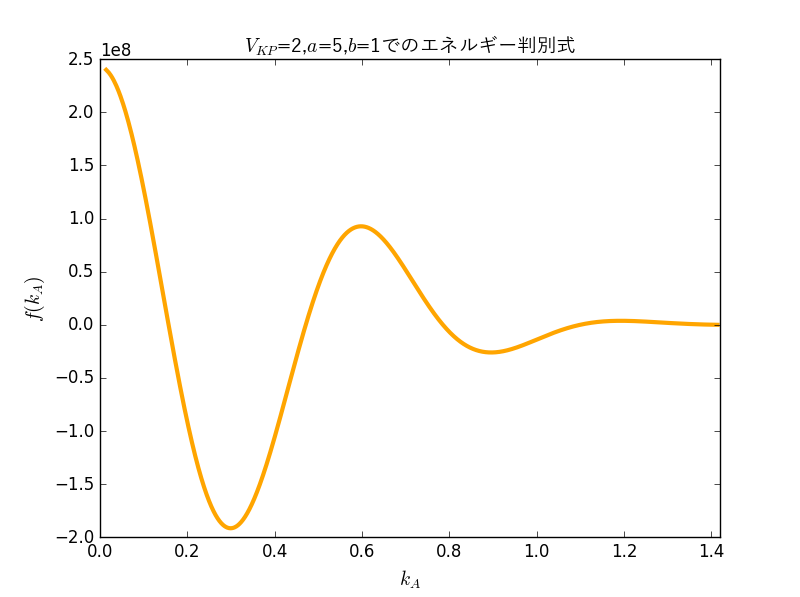
\includegraphics[width=70truemm]{figure_2.png}
             \caption{$k_A$における$V_{KP},a=5,b=1$の判別式}
             \label{BZ1}
    \end{figure}
  \end{block}
\end{frame}

\begin{frame}
    \begin{figure}[h]
            \centering
            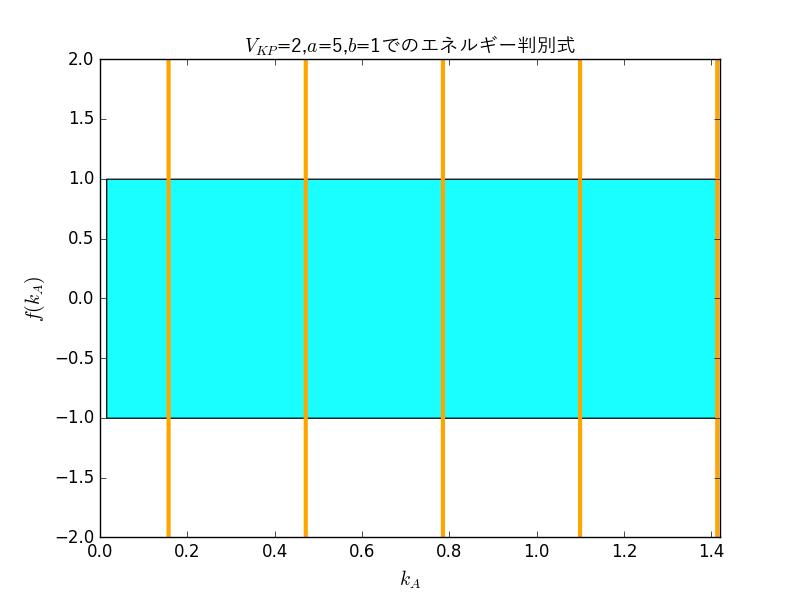
\includegraphics[width=70truemm]{figure_1.png}
            \caption{拡大した判別式}
            \label{BZ2}
    \end{figure}
\end{frame}

\begin{frame}
    \begin{block}{Blochの定理とKronig-Pennyモデルについてのまとめ}
        \begin{itemize}
            \item ハミルトニアンに並進対称性を課すとBlochの定理が成立する
            \item Kronig-Pennyモデルの定常解はエネルギー状態に制限がある
            \item Kronig-Pennyモデルの具体的なエネルギーバンド領域を求めることは難しい
        \end{itemize}
    \end{block}
\end{frame}

\subsection{HunagelとZhangのHeyperdiffusion}
\frame{\insertsubsection}

\begin{frame}
  \begin{block}{ポテンシャルと波束}
    通常の波束の緩和:\eref{SD}\\
    \alert{but}\\
    周期ポテンシャルでは?
  \end{block}
  \begin{block}{Hunagel}
    量子が一点から拡散する状況\\
    $\rightarrow$tight-bindingモデル$\times$point-sourceモデル
  \end{block}
\end{frame}

  \begin{frame}
    \begin{block}{分散}
    $M_{PS}$が\eref{MPS}
    \begin{align}
    P(t) &= \mathrm{e}^{-\Gamma t}\label{source}\\
    M_{PS}(t)&=\int_{0}^{\infty}\:dx\:x^2\int_{0}^{t}\:dt'(-\dot{P}(t'))\delta(x-v(t-t'))\label{variant}\\
    M_{PS}(t)&=v^2\Gamma\int_{0}^{t}\:dt'\mathrm{e}^{-\Gamma t}(t-t')^2\nonumber\\
    M_{PS}(t)&=v^2\left(t^2-\frac{2}{\Gamma}t+\frac{2}{\Gamma^2}-\frac{2}{\Gamma^2}\mathrm{e}^{-\Gamma t} \right)\label{MPS}
    \end{align}
    $t/\Gamma \ll 1$の状況でかっこ内の第一項以外が消える\\
    分散が$t$の2乗に比例して増加していくことを説明できる\\
    2乗に比例しない因子:Heyperballistic
    \end{block}
  \end{frame}

  \begin{frame}
     \begin{block}{Zhang}
      Kronig-Pennyモデルで波束の緩和を計算\\
     分散が時間の2乗に乗らない拡散
      $\rightarrow$Heyperdiffusion
    \begin{figure}[h]
      \centering
      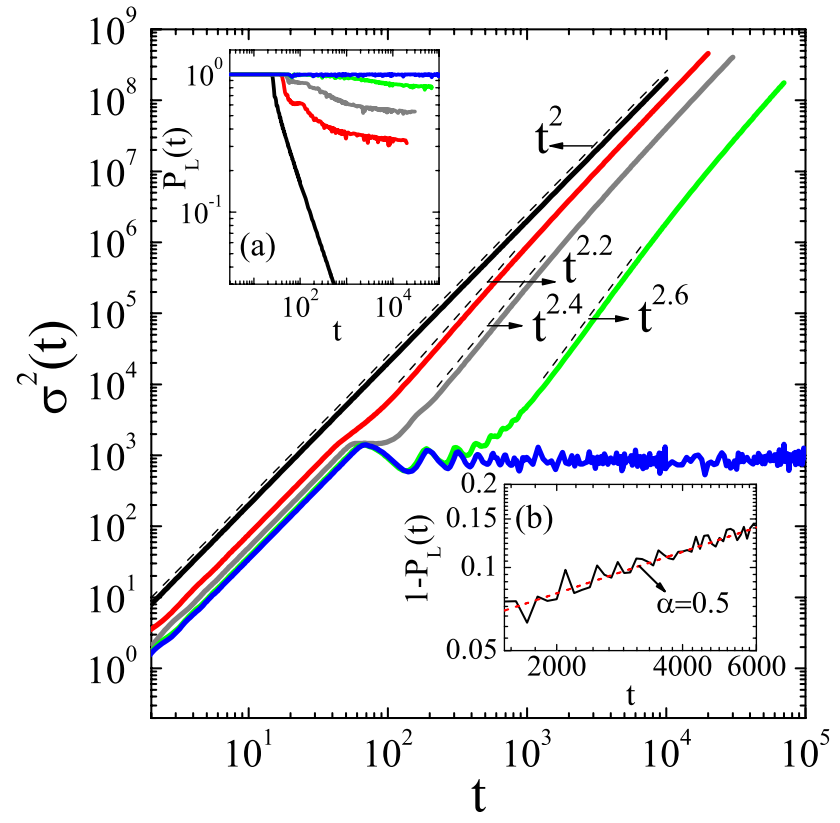
\includegraphics[width=70truemm]{figure_3.png}
      \caption{Zhang PhysRevLett.108(2012)より}
      \label{Zhang}
    \end{figure}
    point-souece近似を使っていない\\
    \alert{but}\\
    Heyperballisticな拡散が起こる\\
    $\rightarrow$Heyperballisticな拡散にpoint-source近似は必須ではない\\
       Zhang:固有状態に関連があるのでは?
    \end{block}
  \end{frame}
%    \begin{itembox}[l]{HunagelとZhangのHeyperdiffusionについてのまとめ}
%        \begin{itemize}
%            \item point-source近似を行うと、ある時間スケールで特異な拡散の挙動が見られる
%            \item Kronig-Pennyモデルの数値計算で類似の状況が予言されている
%            \item Heyperdiffusionには固有状態が影響しているかもしれない
%        \end{itemize}
%    \end{itembox}
%    \chapter{結果}
%    \section{二枚の壁の場合}
%    Kronig-Pennyポテンシャルの簡単な場合として、二枚の壁がある構造を作り、Schrödinger方程式を数値的に計算した。\par
%    ポテンシャルの設定はエネルギーを5、井戸と壁の幅は1に\footnote{
%      すべて原子単位系を採用している。
%    }設定し、波束のパラメータは標準偏差1.5で波数は3のものを入射した。
%    QuantumSketchBookのよる計算の結果、\fref{plt}を得た。
%    \begin{figure}[h]
%      \centering
%      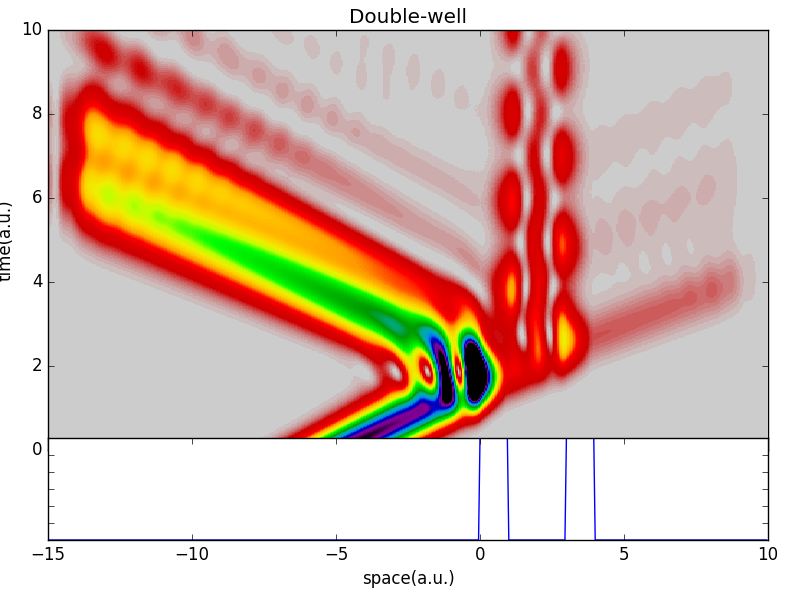
\includegraphics[width=70truemm]{figure_4.png}
%      \caption{確率の時空間分布}
%      \label{plt}
%    \end{figure}
%    この結果から、一度壁に侵入した粒子は反射波と透過波に分かれるが、その後も透過反射を繰り返し、
%    二次的、三次的な波が井戸から放出され続けていることがわかる。
%    そのため、直接反射波と二次、三時反射波の間には時間間隔が存在している。\par
%    また、壁の中央からもう一方の壁の中央までの範囲に粒子が存在する確率を計算したところ、\fref{center1}を得た。\par
%    \begin{figure}[h]
%      \centering
%      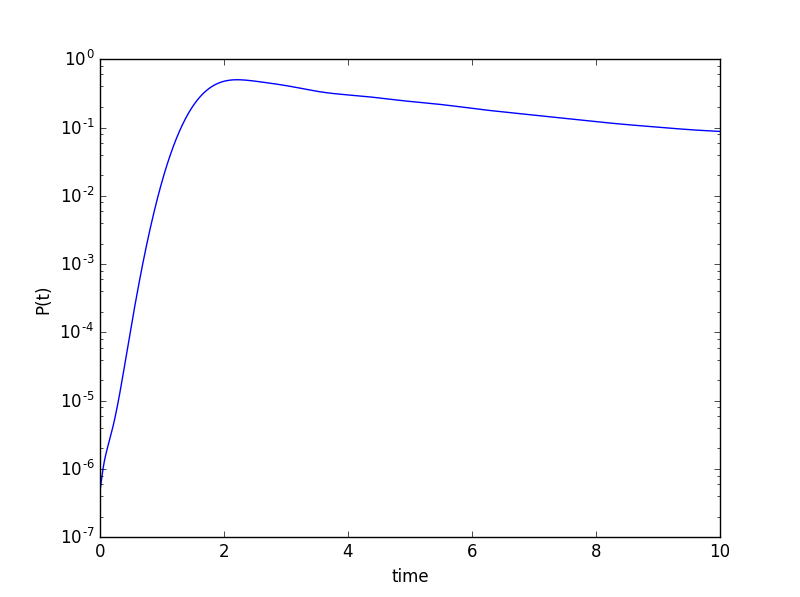
\includegraphics[width=70truemm]{figure_5.png}
%      \caption{井戸付近にいる確率のt=10までの時間推移}
%      \label{center1}
%    \end{figure}
%    波束が侵入したt=2付近から、直線的に確率が減少していることがわかる。
%    この結果から、井戸中央付近に存在している確率は指数関数的に減少していくことが推測される。\par
%    Hunagelによるpoint-source近似の結果がZhangのHeyperdiffusionにも現れた原因として、
%    Kronig-Pennyポテンシャルの井戸部分がpoint-sourceと同様の働きを示したことが考えられる。\par
%    しかし、長時間の計算を行ったところ異なる傾向が見られるようになった。\par
%    それを以下の\fref{center2}に示す。
%    \begin{figure}
%      \centering
%      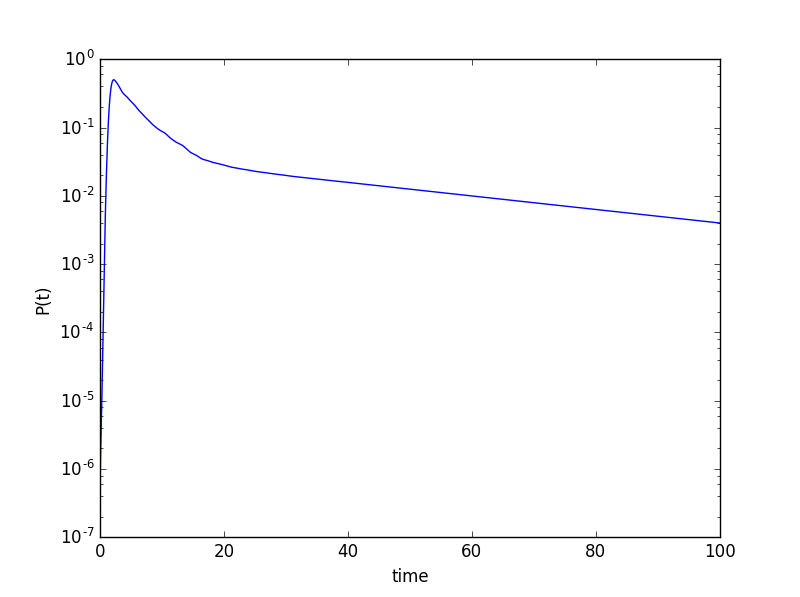
\includegraphics[width=70truemm]{figure_7.png}
%      \caption{井戸付近にいる確率のt=100までの時間推移}
%      \label{center2}
%    \end{figure}
%    t=20頃から傾きが変化していることがわかる。\par
%    この原因として、井戸内の波動関数の振動モードが変化したことが挙げられる。
%    t=100までの時空間分布は\fref{doubleWell}のようになるが、
%    t=10付近では井戸内の波動は両壁付近と井戸中心部の参加箇所に腹が見られる。
%    しかし、t=20付近から井戸中心部の波動が消滅し、壁付近に局在している。\par
%    振動のモードとしてエネルギーが低い状態に落ち込んだため、ポテンシャルの透過確率が低下したと考えられる。
%    \begin{figure}
%      \centering
%      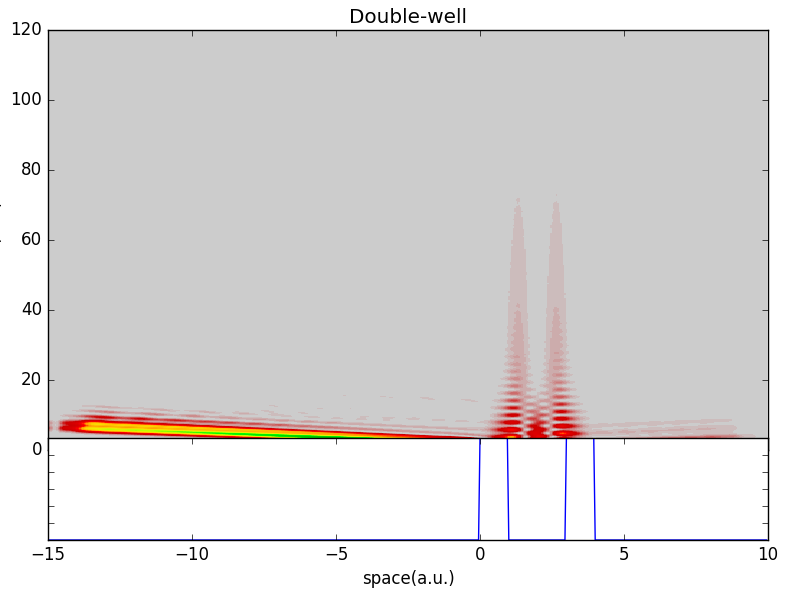
\includegraphics[width=70truemm]{Double-well.png}
%      \caption{t=100までの確率の時空分布}
%      \label{doubleWell}
%    \end{figure}
%    \begin{itembox}[l]{2枚の壁の場合のまとめ}
%      \begin{itemize}
%        \item 反射波は直接のものだけでなく、二次的、三次的な波も現れる
%        \item 井戸周辺の存在確率は指数関数的に減少する
%        \item 減少の指数は時間によって変化する
%        \item 井戸内のモードが関連している可能性がある
%      \end{itemize}
%    \end{itembox}
%    \section{Kronig-Pennyポテンシャル}
%    真空中からKronig-Pennyポテンシャルに入射する場合も同様に計算を行ったところ、\fref{KPfig}を得た。
%    \begin{figure}
%      \centering
%      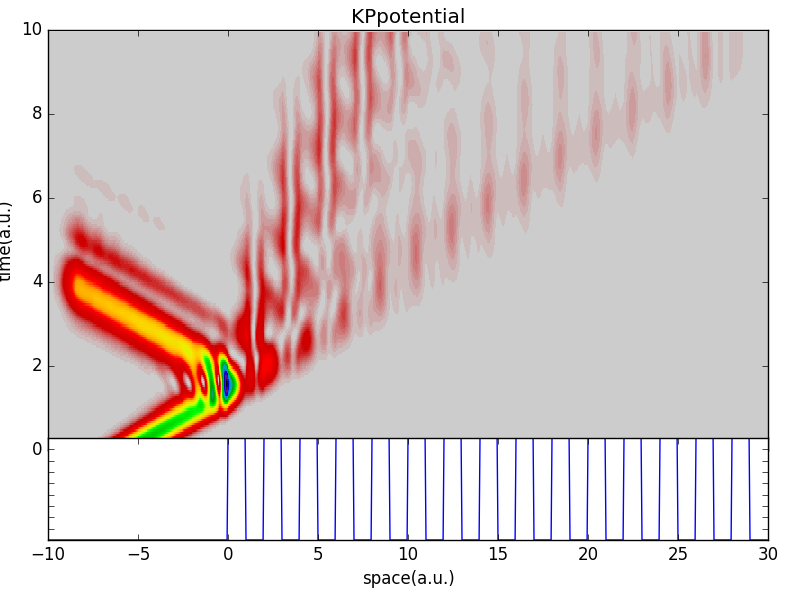
\includegraphics[width=70truemm]{figure_9.png}
%      \caption{Kronig-Pennyポテンシャルにおける確率の時空間分布}
%      \label{KPfig}
%    \end{figure}
%      真空中への反射波は直接反射以外にも、時間的遅れが生じた後、二次反射波や三次反射波が放出されている様子が見える。\par
%      また、Kronig-Pennyポテンシャルに侵入している波は時空間上で複数のすじ状に分布している。\par
%      この現象は、すべての壁を透過した波が1本目のすじに、2回反射した波が2本目のすじになるといったように、
%      反射回数によって波が分離されることによって現れると考えられる。
%      2枚の壁の場合に問題となった振動のモードは、壁の付近が腹になるモードが主で、
%      確率密度が薄くなった1本目のすじの後半付近には壁が節になるモードが現れた。\par
%      \begin{itembox}[l]{Kronig-Pennyポテンシャルのまとめ}
%        \begin{itemize}
%          \item 2枚の壁と同様に反射波には高次のものが現れる
%          \item 透過波に時空間上ですじのようなものが現れる
%        \end{itemize}
%      \end{itembox}
%    \chapter{QuantumSketchBookについて}
%    汎用のコンピュータ言語であるpython3でパッケージQuantumSketchBookを作成し、数値計算を行った。
%    QuantumSketchBookは一体のSchrödinger方程式の解を取得、描画、
%    ハミルトニアンの固有関数と固有値の取得、
%    Nelsonの確率力学に基づいた標本過程の生成を行うことができるパッケージである。
%    生成できる画像の例として、サンプル\fref{sample}を提示する。
%    \begin{figure}
%      \centering
%      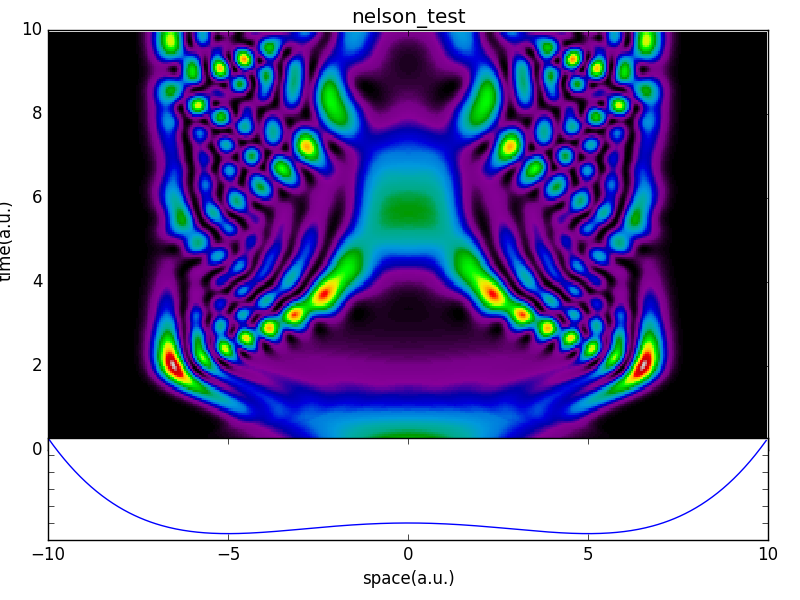
\includegraphics[width=70truemm]{nelson_test.png}
%      \caption{サンプル}
%      \label{sample}
%    \end{figure}
%      この画像は四次ポテンシャルにGauss型波束を置いた場合の時間発展を計算したもので、
%      この分布を元にNelsonの確率過程の標本過程を計算することができる。\par
%      その結果を以下のサンプル\fref{locus}で示す。\par
%    \begin{figure}
%      \centering
%      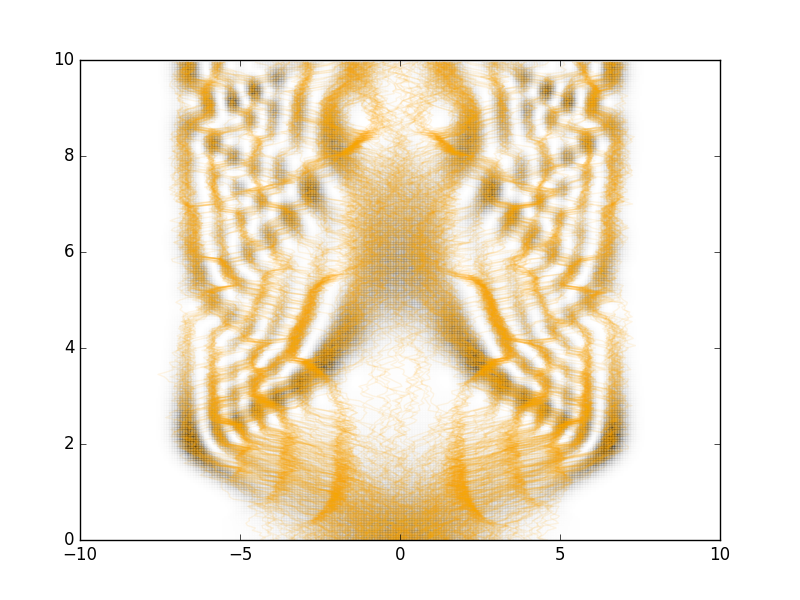
\includegraphics[width=70truemm]{locus_0002.png}
%      \caption{サンプル}
%      \label{locus}
%      \footnotesize{
%        確率密度が高い部分を黒い影として透過させている。
%      }
%    \end{figure}
%    抽象化されたメソッドをつかうため、このような複雑な計算を簡単な入力で計算することができる。\par
%    QuantumSketchBookは主に三種類の部品から作られている。\par
%    一つがSketchBookで、データの保持、他の部品との連携を行う部品である。
%    初心者はこの部品とのやり取りで量子力学の数値計算をこなすことができるようになっている。
%    使い方はpythonのコード内に\\\\
%    \texttt{import \: QuantumSketchBook \: as QSB\\
%            my\_mesh\:=\:QSB.Mesh("位置の最小値、最大値、刻み、時間の最小値、最大値、刻み")\\
%            sb\:=\:QSB.SketchBook(mesh)}\\\\
%    と入力する。\par
%    これにより、\texttt{mesh}の引数を定義域として、様々なデータを格納する準備が整う。
%    初期条件として、デフォルトで$x=0$を中心としたGauss型波束が格納されている。
%    ポテンシャルはデフォルトで$0$の自由粒子状態が格納されている。\par
%    ふたつ目の部品であるPotentialやStateを定義し、SketchBookに渡すことで
%    ポテンシャルや初期条件を設定することができる。\\\\
%    \texttt{
%      my\_potential\:=\:QSB.Potential(mesh\:"位置の関数または各位置のポテンシャルを格納した配列")\\
%      sb.set\_potential(my\_potential)\\\\
%      my\_state\:=\:QSB.State(mesh,\:"位置の関数または各位置の波動関数を格納した配列")\\
%      sb.set\_state(my\_state)\\
%    }\\
%    よく使われるポテンシャルとして、
%    \begin{itemize}
%    \item \texttt{StepPotential()}\: :ステップ型ポテンシャル
%    \item \texttt{BoxPotential()}\: :箱型ポテンシャル
%    \item \texttt{KPPotential()}\: : Kronig-Pennyポテンシャル
%    \item \texttt{UsKPPotential()}\: :右側だけKronig-Pennyポテンシャル
%    \end{itemize}
%    が標準で用意されている。\par
%    また、よく使われる初期条件として\texttt{GaussianState}が用意されている。\par
%    これらの設定ができたら、実際にSchrödinger方程式を解き始められる。\\\\
%    \texttt{
%      import \:QuantumSketchBook\:as\:QSB\\
%      my\_mesh\:=\:QSB.Mesh(-10,\:10,\:0.05,\:0,\:15,\:0.05)\\
%      sb\:=\:QSB.SketchBook(mesh)\\\\
%      my\_potential\:=\:QSB.StepPotential(mesh,\:5,\:0)\\
%      sb.set\_potential(my\_potential)\\\\
%      my\_state\:=\:QSB.GaussianState(mesh,\:-5,\:3,\:3)\\
%      sb.set\_state(my\_state)\\\\
%      sb.solve\_schrodinger\_equation()\\
%    }\\
%    最後の一行で具体的な計算が始まる。\par
%    解は\texttt{sb.solution}と入力すれば取り出すことができる。
%    しかしそれだけはなく、QuantumSketchBookでは簡単な可視化機能も備えている。
%    \texttt{sb.easy\_plot2d()}を実行すれば、解の画像を見ることができる。\\
%    \texttt{
%      import \: QuantumSketchBook \: as \: QSB\\
%      my\_mesh\:=\:QSB.Mesh(-10,\:10,\:0.05,\:0,\:15,\:0.05)\\
%      sb\:=\:QSB.SketchBook(mesh)\\\\
%      my\_potential\:=\:QSB.StepPotential(mesh,\:5,\:0)\\
%      sb.set\_potential(my\_potential)\\\\
%      my\_state\:=\:QSB.GaussianState(mesh,\:-5,\:3,\:3)\\
%      sb.set\_state(my\_state)\\\\
%      sb.solve\_schrodinger\_equation()\\
%      sb.easy\_plot2d(save=True,\:title="test")\\
%    }
%    以上のコードを実行すれば、解を可視化した画像\fref{testfig}が得られる。\\
%    \begin{figure}
%      \centering
%      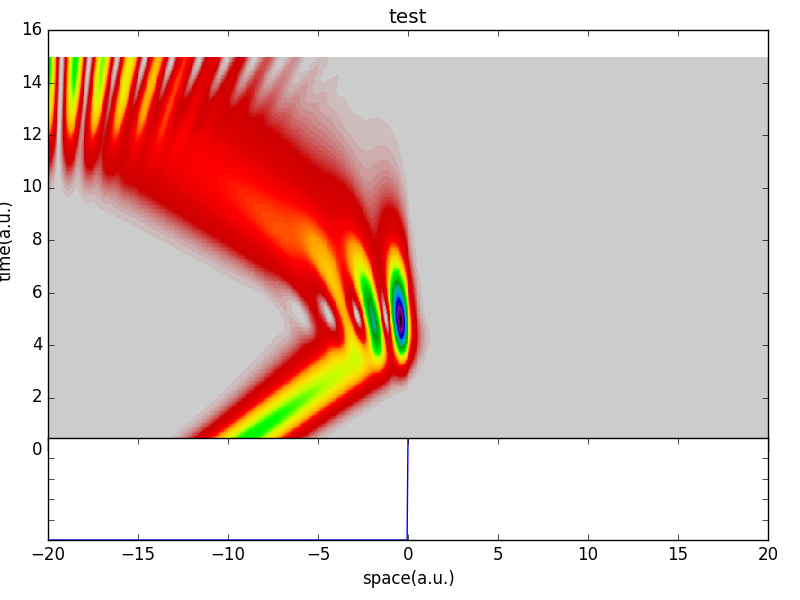
\includegraphics[width=70truemm]{figure_10.png}
%      \caption{テスト}
%      \label{testfig}
%    \end{figure}
%    境界付近で値が不安定になっているが、これは自由端境界条件をつけているためである。\\
%    境界条件は\texttt{sb.solve\_schrodinger\_equation(boundary="free")}といった形で指定できる。
\end{document}
